\documentclass[10pt,
               spanish, %cfr. https://is.gd/n3cszn
               twocolumn,
               openright
               ]{report}

% a4large.sty -- fill an A4 (210mm x 297mm) page
% Note: 1 inch = 25.4 mm = 72.27 pt
% 1 pt = 3.5 mm (approx)
               
\usepackage[paperheight=297mm,
            paperwidth=210mm,
            tmargin=28mm, 
            headheight=0mm, 
            headsep=3mm,
            textheight=250mm,
            footskip=10mm,
            textwidth=160mm,
            bindingoffset=10mm,
            twoside
            ]{geometry}

% paragraph setup
\setlength{\parindent}{0em}
%\setlength{\parindent}{4em}
\setlength{\parskip}{1em}
\setlength{\columnsep}{1em}
%\renewcommand{\baselinestretch}{1.5}

\usepackage[utf8]{inputenc}
\usepackage[spanish]{babel}
\usepackage{enumerate}
\usepackage[pdftex]{graphicx}
\usepackage{csquotes} % quotation
\usepackage[usenames,dvipsnames]{color}
\definecolor{webgreen}{rgb}{0, 0.5, 0} % less intense green
\definecolor{webblue}{rgb}{0, 0, 0.5}  % less intense blue
\definecolor{webred}{rgb}{0.5, 0, 0}   % less intense red
\definecolor{dblackcolor}{rgb}{0.0,0.0,0.0}
\definecolor{dbluecolor}{rgb}{.01,.02,0.7}
\definecolor{dredcolor}{rgb}{0.8,0,0}
\definecolor{dgraycolor}{rgb}{0.30,0.3,0.30}

%\usepackage[math]{iwona}
\usepackage{beton}
\usepackage[T1]{fontenc}

\usepackage{makeidx}
\makeindex % cfr https://en.wikibooks.org/wiki/LaTeX/Indexing

\usepackage[hang, flushmargin]{footmisc}
\usepackage[bookmarks=true,
            bookmarksnumbered=false, % true means bookmarks in 
                                     % left window are numbered                         
            bookmarksopen=false,     % true means only level 1
                                     % are displayed.
            colorlinks=true,
            linkcolor=webred,
            urlcolor=NavyBlue,
            citecolor=OliveGreen]{hyperref}
\usepackage{footnotebackref}

\newcommand{\HRule}{\rule{\linewidth}{1mm}}

\title
{
\HRule
\begin{flushright}
\Large
\textbf{Almirante }\\[4mm]
\huge
\textbf{Blas de Lezo}\\
\end{flushright}
\HRule 
}

\author{\href{https://es.wikipedia.org/wiki/Blas_de_Lezo}{Wikipedia}}

\date{\today}

\begin{document}
\bibliographystyle{alphadin} % Alpadin nos va a permitir añadir hipervínculos a la web
\maketitle
\tableofcontents
\listoffigures

\chapter{Introducción}
%\chapter{Introducción}

\textit{Blas de Lezo y Olavarrieta} (u \textit{Olabarrieta})
\index{Blas de Lezo} (Pasajes, Guipúzcoa, 3 de febrero de
1689---Cartagena de Indias, Nueva Granada, 7 de septiembre de 1741)
fue un almirante español ---conocido por la singular estampa que le
dieron sus numerosas heridas de guerra considerado uno de los mejores
estrategas \index{armada!española} de la historia de la Armada
Española y famoso por dirigir, junto con el virrey Sebastián de
Eslava, la defensa de Cartagena de Indias durante el asedio británico
de 1741 (cfr. \cite{bci}).  \index{Cartagena!de Indias}

Blas de Lezo y Olavarrieta nació en el distrito de Pasajes de San
Pedro (Guipúzcoa) ---por entonces aún parte de San Sebastián--- a
principios de febrero de 1689 y fue bautizado en la iglesia de San
Pedro de la misma localidad el día seis siguiente. Hijo de Pedro de
Lezo y Agustina Olabarrieta, pertenecía a una familia con ilustres
marinos entre sus antepasados, en un pueblo dedicado, prácticamente en
exclusiva, a la mar. Era el tercer hijo del matrimonio, que tuvo ocho,
de los que no todos sobrevivieron a la infancia. Sus padres
pertenecían a la pequeña nobleza local, acomodada, y De Lezo contaba
con algunos antepasados importantes: su tatarabuelo había sido regidor
de la villa a comienzos de siglo, otro había sido obispo de Perú el
siglo anterior y su abuelo había sido capitán y dueño de un galeón. El
mayorazgo le privaba prácticamente de heredar bienes, así que optó por
emprender la carrera militar, como marino.

% \begin{figure}[!hbp]
% \centering
% \mbox{
% \subfigure[Rueda-piñón de un tanque Leclerc.]{
% \label{hph_01}
% 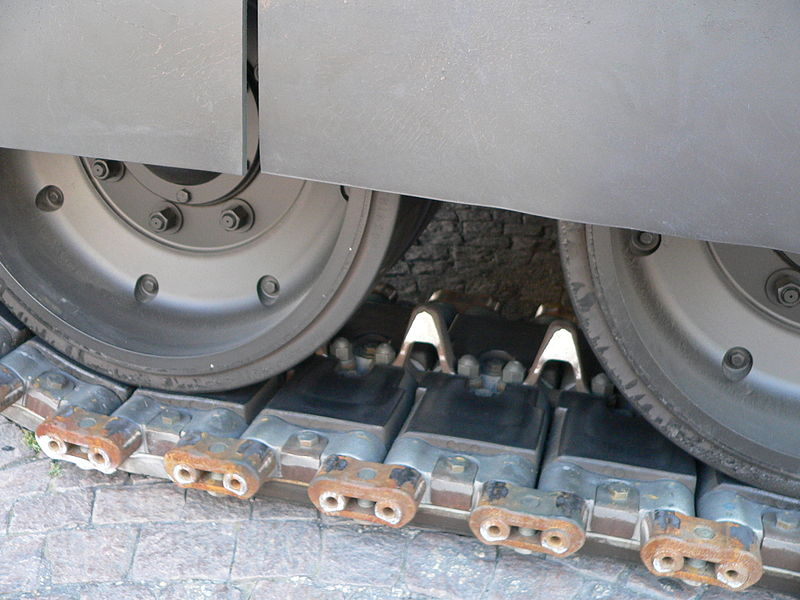
\includegraphics[width=.38\textwidth]{oruga_01.jpg}
% }
% \qquad
% \subfigure[Rueda de rodamentos de un tanque Leclerc.]{
% \label{hah}
% 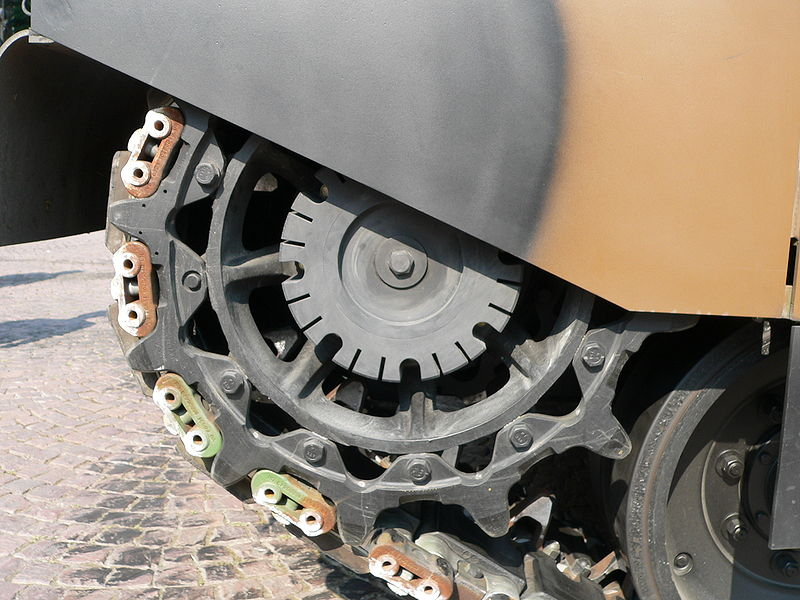
\includegraphics[width=.35\textwidth]{oruga_02.jpg}
% }
% }

% \mbox{
% \subfigure[Mi Carraro durante la carrera ]{
% \label{heh}
% 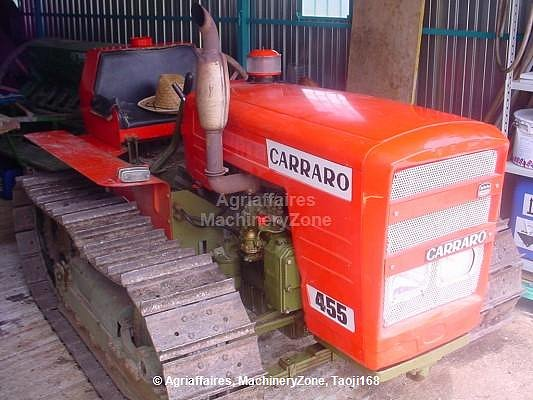
\includegraphics[width=.50\textwidth]{oruga_04.jpg}
% }
% }
% \caption{\label{fig:oruga} Detalles de un vehículo oruga.}
% \end{figure}

\begin{figure}[!hbp]
\centering
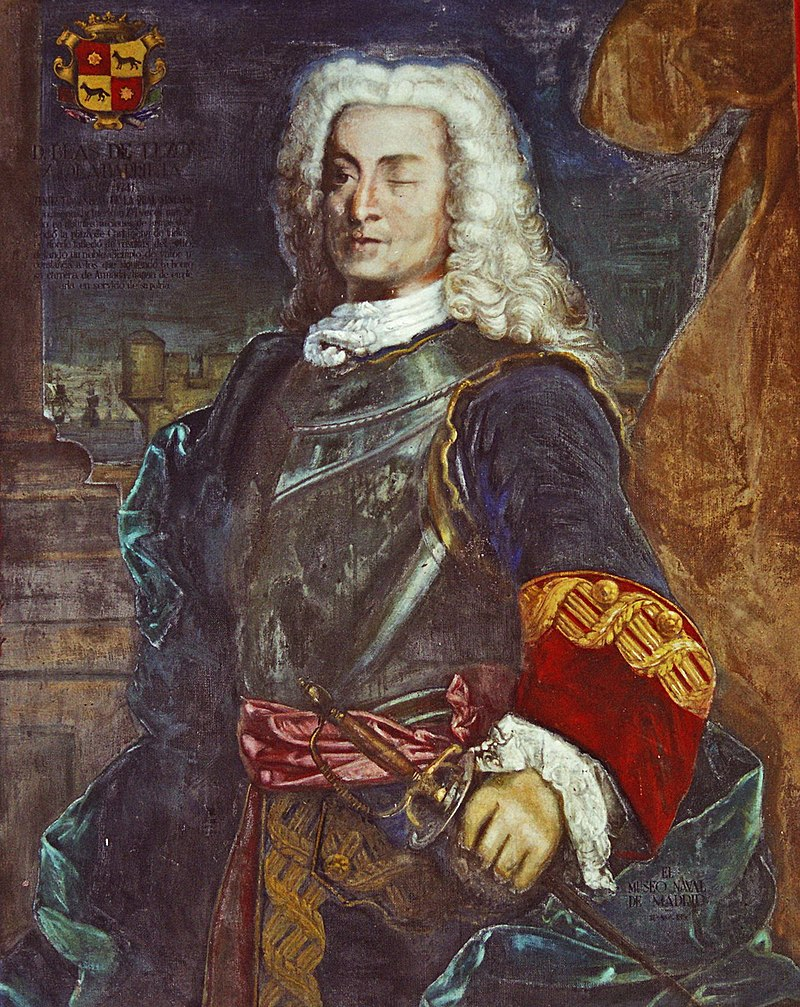
\includegraphics[width=.35\textwidth]{jpg_Don_Blas_de_Lezo_-Museo_Naval-.jpg}
\caption{\label{fig:donBlas} Don Blas de Lezo (Museo Naval de Madrid).}
\end{figure}

Se educó en el Colegio de Francia, una institución educativa para
niños de la baja nobleza de la zona donde recibió la instrucción
básica. En aquel entonces la armada francesa \index{armada!francesa}
era aliada de España en la Guerra de Sucesión, que acaba de empezar al
morir Carlos II sin descendencia. Dado que Luis XIV deseaba el mayor
intercambio posible de oficiales entre los ejércitos y escuadras de
España y Francia, Lezo se embarcó, a sus doce años, en 1702, en la
escuadra francesa ---que, en la práctica, había absorbido a la
española, en estado calamitoso, enrolándose como guardiamarina al
servicio del conde de Toulouse, Luis Alejandro de Borbón, hijo de Luis
XIV.

Se le ofreció ser asistente de cámara de la Corte de Felipe V. Rechazó
este cargo y, una vez recuperado de la pérdida de la pierna, siguió su
servicio a bordo de diferentes buques, tomando parte en las
operaciones que tuvieron lugar para socorrer las plazas de Peñíscola y
Palermo; en el ataque al navío inglés Resolution de setenta cañones
en la costa genovesa, que terminó con la quema de este; así como en
el apresamiento posterior de dos navíos enemigos en el Mediterráneo
occidental, que fueron conducidos a Pasajes y Bayona, todo ello en
1705. El mando de las presas se otorgaba como premio a los oficiales
que se habían distinguido en el servicio, como debió de hacer Lezo en
los combates de ese año.

Marino de reconocido talento y genialidad, cuya brillante carrera
aseguró el dominio marítimo del Imperio Español durante 60 años
más. Sin embargo, aunque las proezas de Blas de Lezo estén a la altura
de los más grandes héroes de la historia, es un personaje
prácticamente olvidado con el que los españoles siempre estaremos en
deuda.
\chapter{Guerra de Sucesión}
%\chapter{Guerra de Sucesión}

La guerra enfrentaba a Felipe de Anjou, apoyado por Francia y nombrado
heredero por el difunto rey español, con el archiduque Carlos de
Austria, apoyado por Inglaterra, ya que esta última temía el poderío
que alcanzarían los Borbones en el continente en caso de unirse las
dos coronas, española y francesa. Para recuperar
Gibraltar\index{Gibraltar|textbf} ---tomado
por las fuerzas anglo-holandesas--- y desbloquear el acceso al
Mediterráneo, franceses y españoles aprestaron una gran armada
(cfr. \cite{qui01,garciarivas}).\index{armada} La escuadra francesa había salido de
Tolón y en Málaga se habían unido a ella algunas galeras españolas
mandadas por el conde de Fuencalada. Frente a Vélez-Málaga se produjo
el 24 de agosto de 1704 la batalla naval más importante del
conflicto. En dicho combate se enfrentaron 96 naves de guerra
franco-españolas (51 navíos de línea, seis fragatas, ocho brulotes y
doce galeras, que sumaban un total de 3577 cañones y 24277 hombres) y
la flota anglo-holandesa, mandada por el almirante Rooke y compuesta
por 53 navíos de línea, seis fragatas, pataches y brulotes con un
total de 3614 cañones y 22543 hombres, dando como resultado al final
de la contienda 1500 y 2719 bajas, respectivamente.

Blas de Lezo participó en aquella batalla batiéndose de manera
ejemplar,\index{Blas de Lezo} hasta que, poco después de comenzar el
combate, una bala de cañón le destrozó la pierna izquierda
(cfr. \cite{qui01}), teniéndosela que amputar, sin anestesia, por
debajo de la rodilla. Debido al valor demostrado tanto en aquel trance
como en el propio combate, fue ascendido en 1704 a alférez de bajel de
alto bordo por Luis XIV, al que el comandante francés había notificado
la bizarría de Lezo. Felipe V le otorgó también una merced de hábito,
que conllevaba una serie de privilegios similares a los de la baja
aristocracia.

\begin{figure}[!hbp]
\centering
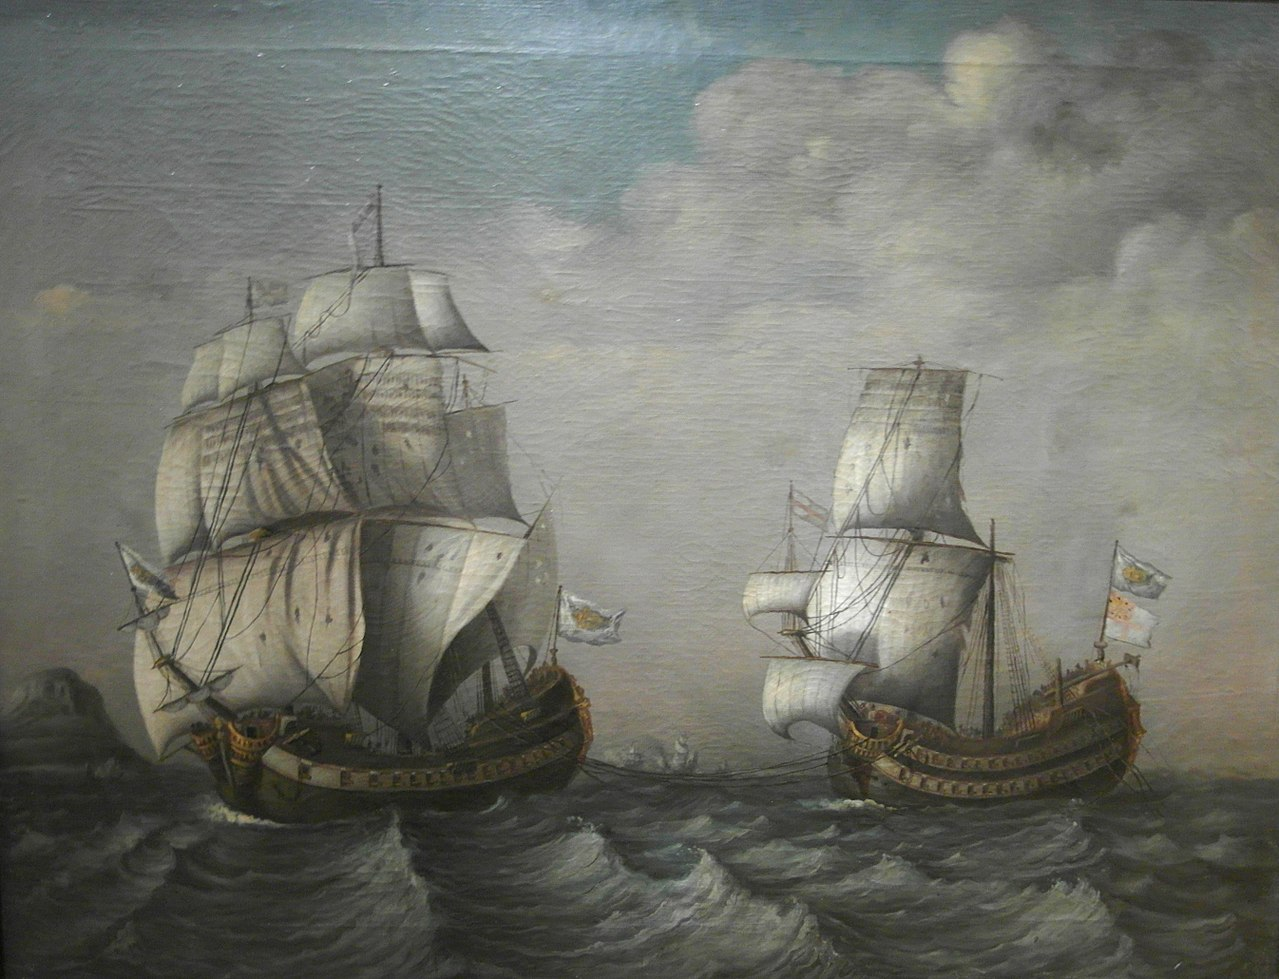
\includegraphics[width=.35\textwidth]{jpg_LaFragataDeBlasDeLezoRemolcandoAlStanhopeHaci1710.jpg}
\caption{\label{fig:fragata} La fragata de D. Blas de Lezo remolcando
al buque británico \textit{Stanhope}.}
\end{figure}

Se le ofreció ser asistente de cámara de la Corte de Felipe V. Rechazó
este cargo y, una vez recuperado de la pérdida de la pierna, siguió su
servicio a bordo de diferentes buques, tomando parte en las
operaciones que tuvieron lugar para socorrer las plazas de Peñíscola y
Palermo; en el ataque al navío inglés Resolution de setenta cañones en
la costa genovesa, que terminó con la quema de este; así como en el
apresamiento posterior de dos navíos enemigos en el Mediterráneo
occidental, que fueron conducidos a Pasajes y Bayona, todo ello en
1705. El mando de las presas se otorgaba como premio a los oficiales
que se habían distinguido en el servicio, como debió de hacer Lezo en
los combates de ese año.

Evidentemente necesitó una larga recuperación y rechazó estar en la
Corte, pues ambicionaba conocer las artes marineras y convertirse en
un gran comandante.

Pero enseguida es requerido por sus superiores y en 1706 se le ordenó
abastecer a los sitiadores de Barcelona al mando de una pequeña
flotilla, parte de la armada \index{armada} que con este fin mandaba
un almirante francés. Realizó brillantemente su cometido, escapando
una y otra vez de las naves enemigas y facilitando el
aprovisionamiento del ejército del mariscal de Tessé. Para ello deja
flotando y ardiendo paja húmeda con el fin de crear una densa nube de
humo que ocultase los navíos españoles, pero además carga ``sus
cañones con unos casquetes de armazón delgada con material incendiario
dentro, que, al ser disparados, prenden fuego a los buques
británicos'' (cfr. \cite{garciarivas}). Los británicos se ven
impotentes ante tal despliegue de ingenio.

Posteriormente se le destacó a la fortaleza de Santa Catalina de
Tolón, donde participó en la defensa de la base naval francesa de la
acometida de la flota del príncipe Eugenio de Saboya. En esta acción y
tras el impacto de un cañonazo en la fortificación, una esquirla le
reventó el ojo izquierdo.

\chapter{Caribe y el Pacífico}
%\chapter{Caribe y el Pacífico}

Terminada la Guerra de Sucesión, se le confió el buque Peibo del
Primer Lanfranco, barco en calamitoso estado. Un año después, en 1716,
partió hacia La Habana con la Flota de Galeones, con la misión
habitual de escoltar a los barcos mercantes que viajaban a América y
la especial de limpiar de naves corsarias las aguas de la región, que
habían realizado algunas presas el año anterior \cite{qui01}. Cumplida
la misión, Lezo regresó a Cádiz, donde en 1720 obtuvo el mando de un
nuevo Lanfranco, de sesenta y dos cañones y también genovés, como su
homónimo, conocido asimismo como León Franco y Nuestra Señora del
Pilar.

Con este nuevo navío se integró en una escuadra hispano-francesa al
mando de Jean Nicolas Martinet ---francés al servicio de la Corona
española--- y Bartolomé de Urdizu ---segundo de Martinet y capitán del
único buque real que se unió a los que aportaban los corsarios
franceses---, que partió en diciembre de 1716 a América con el cometido
de limpiar de corsarios y piratas los llamados Mares del Sur, o lo que
es lo mismo, las costas del Perú. La escuadra estaba compuesta por
parte española por cuatro buques de guerra y una fragata y, por parte
francesa, por dos navíos de línea. Tras diversos retrasos, el
grueso de la flota alcanzó El Callao el 27 de septiembre de 1717.
Urdizu y Lezo, sin embargo, tuvieron problemas para doblar el Cabo de
Hornos y se retrasaron; alcanzaron El Callao finalmente en enero de
1720, cuando ya las autoridades del Perú habían devuelto a Europa a
los franceses por las tensiones entre las dos partes.

Las primeras operaciones de los marinos españoles encargados de la
reforma de la flota virreinal fueron contra los dos barcos, el Success
(70) y el Speed Well (70) del corsario inglés John Clipperton, que
logró evitar a la flota virreinal durante algún tiempo, pero tuvo
finalmente que abandonar la zona \cite{qui01}. La flota pasó entonces
a desempeñar labores de vigilancia y patrulla en la región, que
acabaron por minar la salud de Urbizu. La mayor parte de las labores
de patrulla, dada la mala salud de este, recayeron en Lezo.

Agotado Urbizu, lo sustituyó el 16 de febrero de 1723, Lezo, con el
título de general de la Armada de Su Católica Majestad y jefe de la
Escuadra del Mar del Sur, por entonces de escaso tamaño. Además
del Lanfranco de Lezo, la formaban los navíos Conquistador y
Triunfador y la fragata Peregrina.

En mayo de 1725, se casó con una limeña de la alta sociedad, Josefa
Pacheco de Bustos y Solís, veinte años más joven; la boda la presidió
el arzobispo de Lima, fray Diego Morcillo y Rubio de Auñón, que hasta
el año anterior había sido virrey del Perú y había establecido buenas
relaciones con Lezo.

Para reforzar la flota que mandaba, hizo reparar los navíos de línea
con que contaba, desguazó y vendió la Peregrina, de cara recuperación
y mal adaptada a las aguas de la región e hizo construir otros dos
navíos. A principios de 1725 zarpó para combatir el corso y el
contrabando de acuerdo a los bandos promulgados el año anterior por el
nuevo virrey. Tras algunas semanas de patrulla, Lezo se topó con una
escuadra holandesa de cinco barcos, que aventajaban a la suya en
artillería. Sin arredrarse, la acometió; tras una denodada lucha
logró derribar el palo mayor de la capitana y apresarla, y puso en
fuga al resto de buques. Más tarde, atacó y se apoderó de una flota
inglesa de seis barcos de guerra, de los que se quedó tres para la
escuadra virreinal.

Estos éxitos y el crecimiento de la flota disuadieron a los enemigos
y, paradójicamente, llevaron al enfrentamiento entre el virrey,
marqués de Castelfuerte, que deseaba reducir la flota para ahorrar
gastos una vez que la situación parecía controlada, y Lezo, que se
oponía a ello. La relación entre ellos también había empeorado por el
nombramiento nepotista del sobrino del virrey para el cargo de
tesorero de los ingresos por comercio marítimo, que contravenía las
disposiciones y del que Lezo se quejó. Mal avenido con el virrey, que
trató de desacreditarle mediante una inspección ---juicio de
residencia--- de su labor que no encontró falta en el desempeño del
marino, disgustado por el desmantelamiento de la flota ---el virrey
prefirió armar corsarios que invertir en reforzar la flota--- y con
mala salud por la larga estancia en la región y las insalubres
travesías, en septiembre de 1727 escribió al secretario de Marina,
José Patiño para quejarse y solicitar su retiro. Patiño aceptó que
dejase el mando de la escuadra del Perú y le llamó a España, pero no
permitió que abandonase la Armada, consciente de su valía.64 El 13 de
febrero de 1728, le relevó como jefe de la flota virreinal y le ordenó
regresar a la península ibérica, pero Lezo, enfermo, no pudo hacerlo
hasta el año siguiente; el 18 de agosto de 1730 arribó con su familia
a Cádiz. Tras librarse de una epidemia de vómito negro que aquejaba a
la ciudad gracias a haberse inmunizado en América, acudió a Sevilla a
visitar al rey, que ya mostraba signos de desequilibrio mental; la
audiencia real tuvo lugar a finales de septiembre o principios de
octubre.

\section{Matrimonio y Descendencia}

El 5 de mayo de 1725, había contraido matrimonio en Lima con la dama
criolla Josefa Pacheco de Bustos, natural de Locumba (actual Tacna), e
hija de los también criollos José Carlos Pacheco y Benavides, y María
Nicolasa de Bustos y Palacios. El matrimonio tuvo siete hijos: Blas67
Fernando, nacido en Lima y primer marqués de Ovieco (1726); Josefa
Atanasia, nacida también en Lima (1728); Cayetano Tomás; Pedro
Antonio; Agustina Antonia; Eduvigis Antonia, que profesó como su
hermana mayor como agustina recoleta; e Ignacia, que casó con el
marqués de Tabalosos. Los cinco hijos menores nacieron en la península
ibérica y, de ellos, las dos hermanas menores, en El Puerto de Santa
María.

\chapter{En El Mediterráneo}
%\chapter{En El Mediterráneo}

\section{Jefe de la Escuadra del Mediterráneo}

Estuvo inactivo en Cádiz un año, hasta que el 3 de noviembre de 1731
se lo nombró jefe de la escuadra naval del Mediterráneo. Esta contaba
con tres navíos de línea, entre ellos el Real Familia, de sesenta
cañones y almiranta de Lezo. La escuadra tenía un papel fundamental en
las ambiciones políticas del rey, que deseaba recuperar los
territorios perdidos en la península itálica en los
tratados\index{Tratado} de paz de la guerra de sucesión. En
reconocimiento de sus servicios al rey, este le concedió en 1731 como
estandarte para su capitana la bandera morada con el escudo de armas
de Felipe V, la Orden del Espíritu Santo ---máxima condecoración
francesa--- y la Orden del Toisón de Oro ---más alta condecoración
española--- alrededor y cuatro anclas en sus extremos.

\section{Primeras Misiones en Italia}

Su primera misión fue participar en diciembre de ese año en la escolta
del infante Carlos, que pasaba a Italia a adueñarse de los ducados de
Parma, Toscana y Plasencia. Lezo mandaba una escuadra de veinticinco
navíos, parte de una flota mayor en la que participaban los ingleses.

Al demorarse los genoveses en devolver los dos millones de pesos
pertenecientes a la Hacienda española que se hallaban depositados en
el Banco de San Jorge, Patiño ordenó a Lezo partir a la capital de la
república para reclamarlos. Lezo ancló en aquel puerto con seis navíos
y exigió un inaudito homenaje a la bandera real de España y la
devolución inmediata del dinero. Sus seis buques apuntaban los cañones
al palacio Doria, como amenaza al Senado de la ciudad.  Mostrando el
reloj de las guardias a los comisionados de la ciudad, que buscaban el
modo de eludir la cuestión del pago, fijó un plazo, transcurrido el
cual la escuadra rompería el fuego contra la ciudad.  De los dos
millones de pesos recibidos, medio millón fue entregado al infante don
Carlos y el resto fue remitido a Alicante para sufragar los gastos de
la expedición que se alistaba para la conquista de Orán.

\section{Expedición a Orán}

En junio de 1732, volvió de Cádiz a Alicante para sumarse a esta
expedición.\footnote{Artículo principal:
  \href{https://is.gd/wPfH3B}{Expedición española a Orán}.} El objetivo
de esta era recuperar la plaza, que había estado en manos españolas
desde 1509 hasta 1709, cuando se había perdido durante la guerra de
sucesión. Retomarla era una cuestión de prestigio para la Corona y
un modo de demostrar el renovado poderío militar y naval español con
la nueva dinastía. Lezo quedó como lugarteniente del capitán de la
flota de la expedición, Francisco Cornejo, mientras que José Carrillo
de Albornoz, conde de Montemar, mandaba las tropas de tierra. Lezo
participó en la operación a bordo del Santiago, parte de la flota de
doce navíos de guerra, dos fragatas, dos bombardas, siete galeras,
dieciocho galeotas, doce barcos varios y más de quinientos transportes
que componían la escuadra de la expedición.

El asedio de Orán comenzó el 29 de junio, con el desembarco de los
veintiséis mil hombres de Montemar. Tras varios choques, se apoderaron
de la plaza el 1 de julio. Sofocadas las últimas resistencias, que
habían costado más bajas que la conquista de la ciudad, la expedición
regresó a España el 1 de agosto, dejando una guarnición. El 2 de
septiembre, Lezo estaba de vuelta en Cádiz.

Cuando la expedición marchó creyendo cumplida su meta, Bey Hassan,
señor de Orán hasta la reconquista española, logró reunir tropas,
aliarse con el bey de Argel y sitiarla. Bombardeó el castillo de
Mazalquivir y aplastó una salida de los defensores, en la que
perecieron más de mil quinientos soldados y además murió el gobernador
español, Álvaro Navia Osorio y Vigil. Este aristócrata fue el autor de
``Reflexiones militares'', libro de cabecera de Federico el Grande.
Ante la desesperada situación de la plaza, el 13 de noviembre se
ordenó a Lezo socorrerla. Este partió de inmediato con los barcos
que estaban listos para realizar la travesía: dos navíos de línea,
cinco menores y veinticinco transportes, que llevaban cinco mil
soldados de refuerzo a la guarnición. Tras dos días de navegación
alcanzó Orán, desbarató el acoso de las nueve galeras argelinas, que
se retiraron al llegar la escuadra española y abasteció a la
guarnición.

Decidido a acabar con la amenaza que suponía la flota argelina,
decidió perseguirla. En febrero de 1733 logró finalmente localizar la
capitana de sesenta cañones, que se refugió en la bahía de Mostagán,
defendida por dos castillos fortificados. Ello no arredró a Lezo, que
entró en la bahía tras la nave argelina despreciando el fuego de los
fuertes, logró poner en fuga una galeaza que surgió inesperadamente
para auxiliar a la galera, abordarla, incendiarla y, a continuación,
destruir los castillos. Retornó entonces primero a Orán y luego
Barcelona, donde recogió cuatro regimientos de infantería que trasladó
a África. Luego reanudó la patrulla de la zona, entre Tetuán y Túnez
durante dos meses, hasta que una epidemia que se desató en la escuadra
lo forzó a regresar a la ciudad de Cádiz.

\section{Último Periodo en Cádiz}

Hasta 1737, mantuvo un continuo litigio con el virrey de Perú por el
sueldo que se le adeudaba, que este se negó hasta entonces a pagarle,
aduciendo falta de fondos. Lezo, empero, no pasó apuros económicos,
tanto por la fortuna de su mujer como por los ingresos que obtuvo de
diversos negocios, entre ellos el comercio en plata, oro y esclavos,
que había realizado mediante un representante durante su estancia en
el Perú. Parte de las ganancias las invertía en rentables pagarés y
deuda; a pesar de sus continuos combates con los ingleses, mantuvo una
cuenta en un banco londinense.

El 6 de junio de 1734 ascendió a teniente general de la Armada y se lo
nombró comandante general del Departamento de Cádiz. Tras realizar una
visita a Madrid, dos años más tarde, en 1736, se lo trasladó a El
Puerto de Santa María como comandante general de los galeones,
responsable de la seguridad del comercio transatlántico. Se dispuso a
preparar la escuadra que escoltó a la última Armada de los Galeones
\index{armada!de los galeones} de
la carrera de Indias, la de 1737. Los preparativos se retrasaron tanto
por las distintas dificultades ---aprestar los buques de guerra,
reclutar las tripulaciones, asegurar el matalotaje, etc., que Lezo
suscitó el disgusto de Patiño, que le intimó que los acelerará.
Cuando por fin la flota estuvo lista en noviembre de 1736, tuvo que
esperar a que los barcos mercantes cargasen las mercancías y no pudo
partir hasta el 3 de febrero de 1737. El convoy, formado por ocho
mercantes, dos navíos de registro y los dos navíos de escolta de Lezo,
realizó la travesía sin contratiempos y arribó a Cartagena de
Indias. La familia de Lezo ---por entonces, formada por su esposa y
seis hijos, ya que uno había fallecido--- permaneció en El Puerto de
Santa María y no acompañó al marino a su nuevo destino en América.
\chapter{De Vuelta a América. Cartagena de Indias}
%\chapter{De Vuelta a América. Cartagena de Indias}

Regresó a América con los navíos Fuerte y Conquistador en 1737 como
comandante general de Cartagena de Indias, plaza que tuvo que defender
de un sitio (1741) al que la había sometido el ataque del almirante
inglés Edward Vernon.\footnote{Artículo principal:
  \href{https://is.gd/m45nMc}{Sitio de Cartagena de Indias (1741)}} En
los primeros años en Cartagena, Lezo se encargó de labores de
guardacostas, que debían desbaratar el creciente contrabando, que
acabó precipitando la nueva guerra con el \index{Reino Unido} Reino
Unido. Con este mismo objetivo, creó junto con el gobernador de
Cartagena una compañía de armadores de corso. El contrabando británico
había crecido aprovechando las concesiones comerciales que el Reino
Unido había obtenido en el Tratado de Utrecht:\index{Tratado!de
  Utrecht} al comercio legal ---quinientas toneladas ampliadas a mil
en 1716, se unieron pronto los contrabandistas, que amenazaban el
comercio español y trataban de no pagar los derechos (impuestos) a la
Corona. A pesar de la renuencia del Gobierno británico a enfrentarse a
España y favorecer así su acercamiento a Francia, las quejas de los
comerciantes afectados por las actividades de los guardacostas y el
debilitamiento del gabinete de Horace Walpole acabaron por aumentar la
tensión entre los dos países y condujeron finalmente a la guerra.

\begin{figure}[!hbp]
\centering
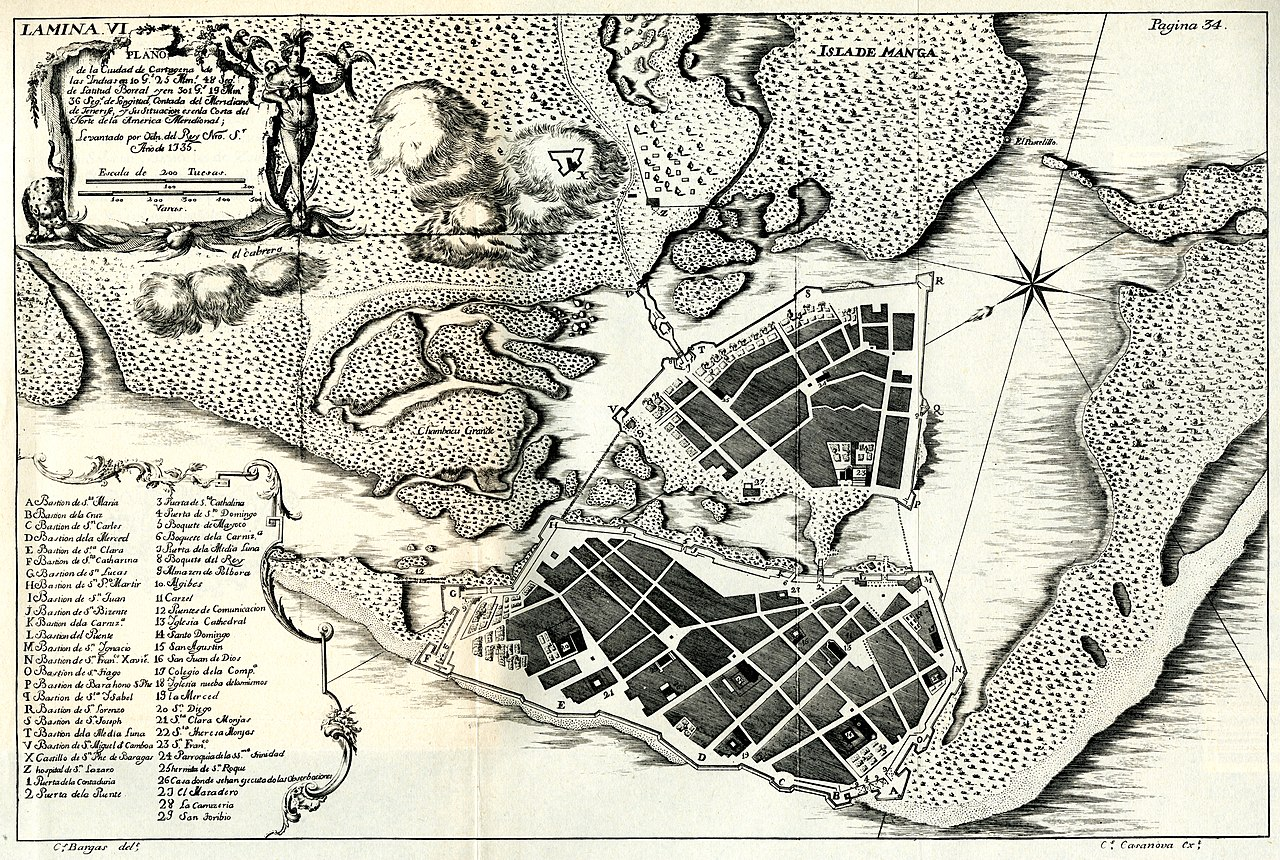
\includegraphics[width=.35\textwidth]{jpg_Plano_de_Cartagena_de_las_Indias_(1735).jpg}
\caption{\label{fig:planoCartagena} Plano de Cartagena de las Indias
  realizado en 1735 y publicado en la obra Relación histórica del
  viaje a la América meridional, de Jorge Juan y Antonio de Ulloa.}
\end{figure}

La justificación de los británicos para iniciar un conflicto con
España fue, entre otros muchos incidentes, el apresamiento de un barco
mercante mandado por Robert Jenkins \index{Jenkins} cerca de la costa
de Florida \index{Florida} en 1731. Juan de León Fandiño apresó el
barco y supuestamente cortó la oreja de su capitán al tiempo que le
decía: «Aquí está tu oreja: tómala y llévasela al rey de Inglaterra,
para que sepa que aquí no se contrabandea». A la sazón, el tráfico de
ultramar español se componía en gran parte del contrabando.

Rechazado en La Guaira el 22 de octubre de 1739, de la que había
pensado apoderarse sin encontrar resistencia, Vernon conquistó la
plaza de Portobelo (Panamá) en noviembre, y desafió a Lezo, a lo que
el marino español contestó:

\begin{displayquote}
{[\ldots]} puedo asegurar a V. E. que si me hubiera hallado en Portobelo
para impedírselo, y si las cosas hubieran ido a mi satisfacción, aun
para buscarle en cualquier otra parte, persuadiéndome que el ánimo que
faltó a los de Portobelo, me hubiera sobrado para contener su cobardía
[en referencia a los defensores del lugar, que la entregaron sin
resistencia].
\end{displayquote}

A continuación y de acuerdo al plan trazado, que los españoles
conocían por los informes de un espía que trabajaba en Jamaica, Vernon
\index{Vernon} se dirigió \index{Cartagena!de Indias|textbf} en
marzo de 1741 contra Cartagena. Antes había realizado dos ataques
exploratorios, con escasas fuerzas, en marzo y mayo de 1740, que Lezo
rechazó.

La flota británica sumaba dos mil cañones dispuestos en casi ciento
ochenta barcos, entre navíos de tres puentes (ocho), navíos de línea
(veintiocho), fragatas (doce), bombardas (dos) y buques de transporte
(ciento treinta), y en torno a treinta mil combatientes entre marinos
(quince mil), soldados (nueve mil regulares y cuatro mil de las
milicias norteamericanas) y esclavos negros macheteros de Jamaica
(cuatro mil).103 Las defensas de Cartagena incluían tres mil hombres
entre tropa regular (unos mil setecientos ochenta), milicianos
(quinientos), seiscientos indios flecheros traídos del interior, más
la cuantiosa marinería y tropa de desembarco de los seis navíos de
guerra de los que disponía la ciudad (ciento cincuenta hombres): el
Galicia, que era la nave capitana, el San Felipe, el San Carlos, el
África, el Dragón y el Conquistador. Tras tomar algunas de las
defensas de la ciudad, el asalto británico al castillo San Felipe de
Barajas, el último baluarte importante que la defendía, fracasó el 20
de abril; con gran parte de la tropa enferma, grandes bajas sufridas
en los combates y la llegada de la época de lluvias, los británicos
optaron por destruir las defensas a su alcance y abandonar el
asedio.

\begin{figure}[!hbp]
\centering
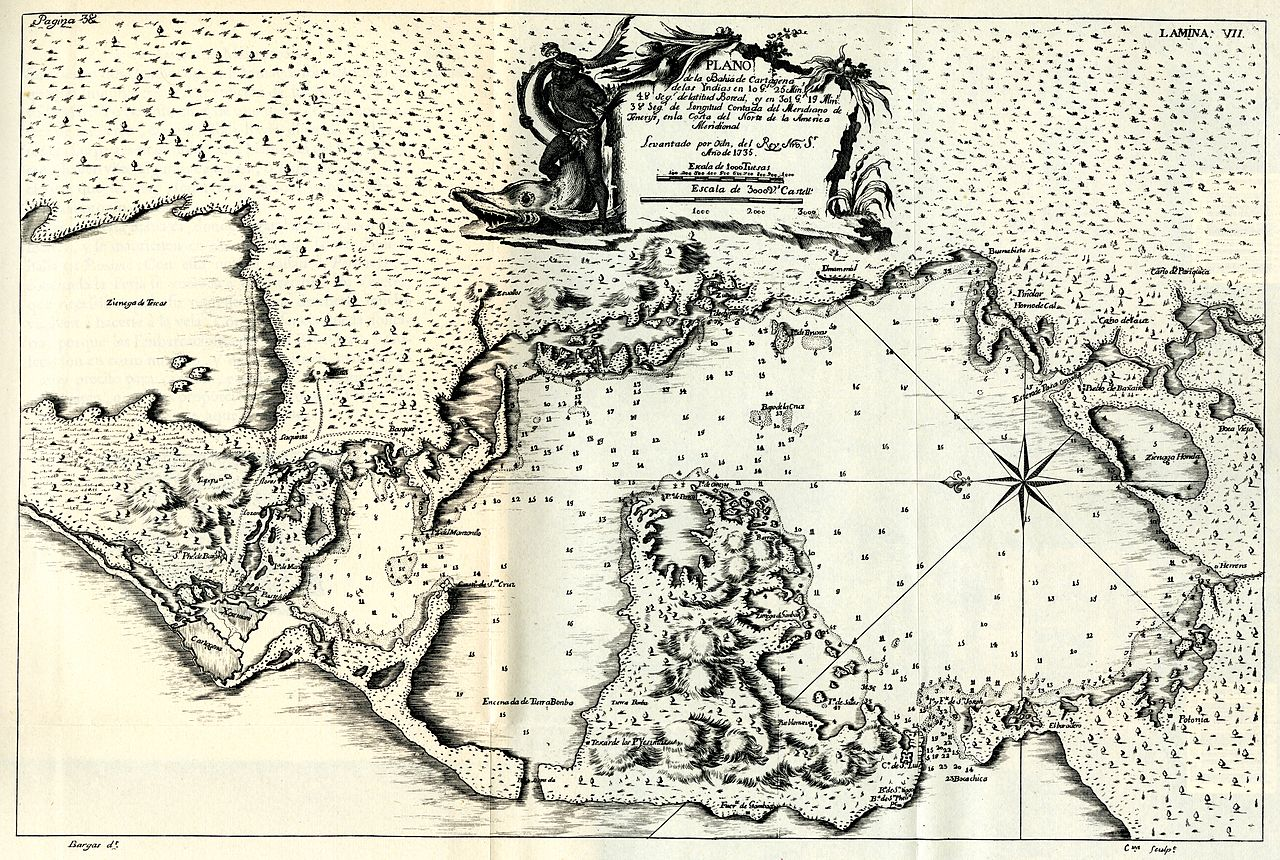
\includegraphics[width=.35\textwidth]{jpg_Plano_de_la_Bahia_de_Cartagena_de_las_Indias_(1735).jpg}
\caption{\label{fig:planoBahiaCartagena} Plano de la Bahía de
  Cartagena de Indias realizado en 1735 y publicado en la Obra
  Relación histórica del viaje a la América meridional, de Jorge Juan
  y Antonio de Ulloa.}
\end{figure}

\index{Cartagena!de Indias}
Las pérdidas británicas fueron graves: unos cuatro mil quinientos
muertos, seis barcos perdidos y entre diecisiete y veinte muy
dañados. Estas últimas obligaron al Gobierno británico a concentrar
sus fuerzas en las defensa de la metrópoli, el Atlántico septentrional
y el Mediterráneo, y a desechar nuevas campañas en las colonias
españolas en América. La derrota en Cartagena desbarató los planes
británicos para la campaña y permitió que continuase el dominio
español en la región durante varias décadas más. Los ingleses, que
contaban con la victoria, se habían precipitado a acuñar monedas y
medallas para celebrarla.108 Dichas medallas decían en su anverso:
«Los héroes británicos tomaron Cartagena el 1 de abril de 1741» y «El
orgullo español humillado por Vernon».

\chapter{Muerte y Castigo Póstumo}
%\chapter{Muerte y Castigo Póstumo}

\begin{figure}[!hbp]
\centering
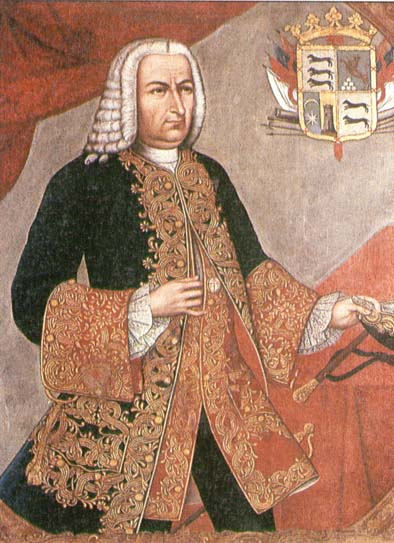
\includegraphics[width=.35\textwidth]{jpg_Sebastian_de_Eslava.jpg}
\caption{\label{fig:eslava} Sebastián de Eslava, virrey de Nueva
  Granada y responsable de la defensa de Cartagena de Indias. Militar
  veterano y ambicioso político, mantuvo un tensa relación con Lezo
  que llevó finalmente a pedir su castigo por sus acciones durante el
  asedio de la ciudad, que obtuvo cuando Lezo ya había fallecido.}
\end{figure}

El 4 de abril, el día que los británicos habían comenzado el bombardeo
sistemático del castillo de San Luis de Bocachica, uno de los que
protegía la ciudad, una bala de cañón había impactado en la mesa del
Galicia en torno a la que estaban reunidos los mandos españoles en
junta de guerra. Las astillas de la mesa hirieron en el muslo y en una
mano a Lezo; la infección de estas heridas le acabó causando la
muerte. La mala relación entre Lezo y el virrey Sebastián de Eslava,
jefe de la plaza y responsable de su defensa, se agudizó una vez
levantado el cerco británico. El primero había abogado constantemente
por adoptar medidas más ofensivas y por acosar al enemigo, mientras
que el segundo había mantenido una actitud más prudente y defensiva,
que para el marino pareció inactividad y desidia en la defensa.

Lezo, cada vez más enfermo, apenas abandonó su residencia a partir del
20 de mayo y mantuvo una guerra epistolar con el virrey, tratando de
defender su actuación durante el asedio, por la que el virrey llegó a
solicitar y obtener el castigo del rey para el marino.116 Lezo intentó
que se reconociese su carrera mediante la obtención de un título
nobiliario, petición para la que recabó el apoyo de José Patiño y de
parte de sus compañeros de armas de la Armada,\index{armada} pero que
el rey, que había recibido los informes desfavorables del virrey y de
otros adversarios de Lezo, rechazó. Blas de Lezo \index{Blas de Lezo}
falleció en Cartagena de Indias \index{Cartagena!de Indias} de «unas
calenturas, que en breves días se le declaró tabardillo» a las ocho de
la mañana del 7 de septiembre. Fue el único de los principales
protagonistas del asedio de Cartagena que no obtuvo recompensa alguna
por sus acciones. Su destitución como jefe del apostadero y la orden
de que regresase a la península ibérica para ser reprendido se aprobó
el 21 de octubre. El rey Carlos III recompensó al hijo de Lezo por las
acciones de su padre, nombrándolo marqués de Ovieco en 1760. Se
desconoce dónde fue enterrado, ya que las fuentes indican distintos
lugares posibles: la iglesia de la Orden Tercera, la capilla de la
Vera Cruz, aneja al convento de San Francisco, o la catedral de
Cartagena.

\section{El Puerto de Santa María y Blas de Lezo}

La estancia de los Lezo en El Puerto de Santa María tuvo varias
fechas. El almirante ya había estado en 1719-20 y en 1730 en Cádiz. De
allí partió, ya viviendo en El Puerto de Santa María, el 3 de febrero
de 1737 hacia Cartagena dirigiendo la que sería la última carrera de
Indias y donde encontraría, como ya se ha reflejado, su fatal destino.

Tras las investigaciones realizadas en los padrones de la época de la
iglesia Mayor Prioral portuense, se ha constatado que Blas de Lezo, su
mujer, sus hijos y un criado afroamericano llamado Antonio Lezo,
vivieron desde 1736 en una casa de la calle Larga, para ser más
exactos en Larga, 70, hoy reconvertida en apartamentos de
alquiler. Tras su muerte, su viuda ---conocida en la localidad como «La
Gobernadora»--- y sus hijos permanecieron en ella hasta la muerte de
ésta el 31 de marzo de 1743.

Josefa Pacheco fue enterrada en el convento de Santo Domingo, sito en
la calle del mismo nombre. A partir de esta fecha, los descendientes
de Blas de Lezo desaparecen de los padrones portuenses.

Durante su residencia en la ciudad, el Cabildo Municipal, siendo
conocedor del prestigio del almirante, hizo a su familia diferentes
concesiones, entre las que destacó una toma de agua para la casa.

Hasta hace pocos años, la ciudadanía portuense siguió llamando a la
mansión casa de «La Gobernadora».
\chapter{Su Memoria}
%\chapter{Su Memoria}

La Real Armada Española \index{armada!española} honra la memoria de
Blas de Lezo \index{Blas de Lezo}con el mayor honor que puede
rendirse a un marino español: tiene por costumbre inveterada que uno
de sus buques lleve su nombre. El último así bautizado es una fragata
de la clase Álvaro de Bazán: la Blas de Lezo (F-103). Anteriormente
portaron dicho nombre un cañonero de la clase Elcano, llamado General
Lezo, que en 1898 se encontraba en Filipinas, aunque no llegó a
participar en los combates al tener las calderas desmontadas, el
crucero Blas de Lezo, que se perdió en 1932 al tocar un bajío frente a
las costas de Finisterre y un destructor procedente de la ayuda
estadounidense, el Blas de Lezo (D-65). La Armada Colombiana
\index{armada!colombiana} también tuvo un buque con el nombre del
almirante, el ARC Blas de Lezo (BT-62), un petrolero de clase
Mettawee, adquirido a la Armada de los Estados Unidos \index{armada !
  de EEUU} el 26 de noviembre de 1947 y dado de baja en enero de 1965.

\begin{figure}[!hbp]
\centering
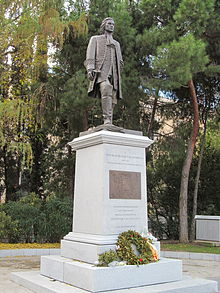
\includegraphics[width=.35\textwidth]{jpg_Blas_de_Lezo_00.jpg}
\caption{\label{fig:donBlas01} Estatua en honor del teniente general
  de la Armada Blas de Lezo en la plaza de Colón en Madrid realizada
  por Salvador Amaya.}
\end{figure}

El 12 de marzo de 2014 se inauguró en el Paseo de Canalejas de la
ciudad de Cádiz el primer monumento dedicado a Blas de Lezo en
España. Al acto acudieron el embajador de Colombia en España y un
almirante de la Armada Española.\index{armada!española} En la
fachada de la Diputación Foral de Guipúzcoa, situada en San Sebastián,
se encuentra desde 1885 un busto de Blas de Lezo, oriundo de Pasajes.

El 15 de noviembre de 2014 el rey Juan Carlos inauguró en los jardines
del Descubrimiento de la plaza de Colón de Madrid una escultura en
bronce de 3,5 metros ---7 metros en total contando con el pedestal---
con la efigie del almirante, muy próxima a la de otros dos marinos
ilustres de la Armada Española como fueron Cristóbal Colón y Jorge
Juan y Santacilia. El monumento fue sufragado íntegramente por
suscripción popular con las aportaciones que un millar de ciudadanos
de todos los rincones de España hicieron a la Asociación Monumento a
Blas de Lezo. \index{Blas de Lezo} Cuatro días después el Ayuntamiento
de Barcelona aprobó una moción con los votos de CiU, ICV, ERC y DCst,
y con la abstención del PSC, en la que se pedía al Ayuntamiento de
Madrid que retirara la estatua por haber participado Blas de Lezo en
el bombardeo de Barcelona durante la Guerra de Sucesión Española. La
petición fue rechazada en rueda de prensa por el ayuntamiento de la
capital.

Existe una placa en su honor en el Panteón de Marinos Ilustres en San
Fernando (Cádiz), donde reposan otros héroes de la Armada
Española. \index{armada!española} También existe una maqueta de la
batalla de Cartagena de Indias \index{Cartagena!de Indias} en la
Academia de Ingenieros de Hoyo de Manzanares (Madrid). Análogamente,
en el Museo Naval de Cartagena de Indias se exhibe un conjunto de
maquetas con detalle de las fortificaciones de aquella bahía y que
describen el sitio de la ciudad por el almirante Vernon, la defensa
organizada por Don Blas de Lezo, \index{Blas de Lezo} y su victoria
sobre el inglés.

Existen calles con su nombre en las ciudades de Valencia, Málaga,
Alicante, Cartagena de Indias, Las Palmas de Gran Canaria, San
Sebastián, Cádiz, Huelva, Fuengirola, Rentería, Irún, Pasajes ---su
localidad natal, y finalmente, tras una recogida de firmas, el 28
de abril de 2010 se aprobó dedicarle una avenida en la capital de
España, Madrid.

Sin embargo, aunque las proezas de Blas de Lezo \index{Blas de Lezo}
están a la altura de los más grandes marinos de la historia, es un
personaje histórico no suficientemente reconocido, ni su biografía
merecidamente divulgada.133 Por esa razón, la empresa española
DL-Multimedia está preparando un documental sobre su vida para los
canales Historia y Odisea.

Blas de Lezo \index{Blas de Lezo} es, al contrario, un reconocido
héroe en Cartagena de Indias, que le rinde homenaje de varias maneras:
barrios, avenidas y plazas le conmemoran en sus nombres; y su estatua
frente al castillo San Felipe de Barajas mantiene vivo entre los
cartageneros el recuerdo del defensor de su ciudad. El 5 de noviembre
de 2009, en Cartagena de Indias, se dio cumplimiento a un deseo de
Blas de Lezo, que en su testamento pedía que un grupo de españoles
pusiese una placa que conmemorase aquella victoria. En la inscripción
se puede leer:

\begin{displayquote}
  Homenaje al Almirante D. Blas de Lezo y Olavarrieta. Esta placa se
  colocó para homenajear al invicto almirante que con su ingenio,
  valor y tenacidad dirigió la defensa de Cartegena de Indias. Derrotó
  aquí, frente a estas mismas murallas, a una armada británica
  \index{armada!británica} de 186 barcos y 23.600 hombres, más 4000
  reclutas de Virginia. Armada aún más grande que la Invencible
  Española que los británicos habían enviado al mando del Almirante
  Vernon para conquistar la ciudad llave y así imponer el idioma
  inglés en toda la América entonces española. Cumplimos hoy juntos,
  españoles y colombianos, con la última voluntad del Almirante, que
  quiso que se colocara una placa en las murallas de Cartagena de
  Indias que dijera: Aquí España derrotó a Inglaterra y sus
  colonias. Cartagena de Indias, marzo de 1741.
\end{displayquote}

Asimismo, el 21 de noviembre de 2009 se descubrió para su memoria una
placa en la calle Larga nº 70 del Puerto de Santa María, ciudad donde
residió Blas de Lezo antes de librar la batalla de Cartagena y donde
nacieron algunos de sus hijos. En dicho acto se estrenó la marcha
militar Almirante Blas de Lezo, compuesta para la Real Armada por
Joaquín Drake García, e interpretada por la Banda de Música del Tercio
Sur (Infantería de Marina). Presidieron el acto el Almirante de la
Flota, el Alcalde de la ciudad y la presidente del Club de Mar Puerto
Sherry. La lápida reza: «En 1736 vivió en este lugar junto a su
familia el Teniente General de la Armada D. Blas de Lezo y
Olavarrieta, insigne e invencible marino, héroe de la Batalla de
Cartagena de Indias en la que la flota inglesa sufrió una humillante
derrota en el año 1741. La ciudad del Puerto de Santa María en
homenaje a su memoria. 21 de noviembre de 2009».


\nocite{alo,arc,ber,fer,mar,qui,rod,smo}

\bibliography{/Users/fmgo/MEGA/base_bib_latex/blasLezo,/Users/fmgo/MEGA/base_bib_latex/mediaCites}

\printindex

\end{document}